% !TEX root = ../notes_template.tex
\chapter{Spin Locks and Contention}\label{chp:spin_locks_contention}
\minitoc

\section{Peterson revisited}
Recall the \verb|PetersonNaive| 2-threaded starvation-free lock algorithm introduced in Section \ref{sec:PetersonLock}. It doesn't work in practice, despite our proof of correctness. To show this, consider the following experiment (in code block \ref{code:naive_peterson_experiment}): write a simple program where two threads repeatedly acquire the \verb|PetersonNaive| lock, increment a shared counter, and release the lock. If each thread does this acquire-increment-release process, say 500,000 times, then the counter should read 1,000,000 at the end. Let's see what happens in practice.

\makebox[\linewidth]{\rule{17cm}{0.4pt}}
{\centering \label{code:naive_peterson_experiment}
\begin{verbatim}
#include "Peterson.hpp"

int main() {
    int counter = 0;
    PetersonNaive mutex;

    auto f = [&mutex, &counter]() {
        for (int i = 0; i < 500000; i++) {
            mutex.lock();
            counter++;
            mutex.unlock();
        }
    };

    std::thread thread1(f);
    std::thread thread2(f);

    thread1.join();
    thread2.join();

    std::cout << "Final result: " << counter <<  std::endl;
    return 0;
}
\end{verbatim}
\captionof{Code}{If PetersonNaive provided mutual exclusion as expected, then the output should be 1000000. However, I got 988,495 (exact output may vary from run to run).}
\makebox[\linewidth]{\rule{17cm}{0.4pt}}
}

\section{Test-and-Set operation}
One of the most basic \textit{read-modify-write} (RMW) operations is test-and-set. It was the principal synchronization instruction used in the earlier multiprocessor architectures.

\begin{algorithm}[H]
    \SetKwInOut{Input}{input}
    \SetKwInOut{Output}{output}
    \Input{Binary value $x$}
    \Output{Binary value}
    \BlankLine
    $t \leftarrow x$;
    
    $x \leftarrow $ TRUE;
    
    \Return $t$;
    \caption{Test-and-Set operation. All of the following instructions occur in a single atomic step.}
    \label{alg:testAndSet}
\end{algorithm}

\subsubsection{Implementing a spin lock using the test-and-set operation}
Declare a binary \verb|flag| field that is set to true if and only if the lock is currently held by some thread. Then the \verb|lock()| method would call \verb|testAndSet(flag)| in a loop, and break once the return value is FALSE. The \verb|unlock()| method simply \verb|set(flag, FALSE)|. See Code \ref{code:TAS_lock} for an implementation.

\makebox[\linewidth]{\rule{17cm}{0.4pt}}
{\centering \label{code:TAS_lock}
\begin{verbatim}
#include <atomic>

class TASlock
{
public:
    void lock() {
        while (flag.exchange(true)) {}
    }

    void unlock() {
        flag.store(false);
    }

private:
    std::atomic_bool flag{false};
};
\end{verbatim}
\captionof{Code}{Implementing a lock based on the test-and-set operation.}
\makebox[\linewidth]{\rule{17cm}{0.4pt}}
}

\section{Array-based Locks}
What is the main shortcoming of the \verb|TTASlock|? It has excess \textit{cache-coherence traffic}.

\begin{definition}[Cache-coherence traffic]
    Consider multiple threads reading from a shared location, each having a locally cached copy of the value. Suppose the value at that shared location changes. That means the locally cached copy of each thread has become \textit{invalidated}. Thus, all threads must reload the value from memory into their cache.
\end{definition}

Thus, one way to implement a better-performing spin lock is \textit{local spinning}, where each thread spins on a different location. We can do this with an array-based lock.

\subsection{Array-based Lock}
The algorithm is simple. \verb|ALock| has a boolean array \verb|ready| with one entry for each thread. It has a shared counter \verb|tail| specifying the index of the last entry in the queue. Each thread will get a \textit{thread-local} "slot" number, which the thread will use to index into the boolean array. A thread is allowed to enter its critical section when \verb|ready[slot]| == TRUE.

\makebox[\linewidth]{\rule{17cm}{0.4pt}}
{\centering \label{code:Alock}
\begin{verbatim}
#ifndef ALOCK_HPP
#define ALOCK_HPP

#define MAX_NO_THREADS 8

class ALock {
public:
    ALock() {
        ready[0] = true;
    }

    void lock() {
        slot = (tail++) % MAX_NO_THREADS;
        while (!ready[slot]) {}
    }

    void unlock() {
        ready[slot] = false;
        ready[(slot+1) % MAX_NO_THREADS] = true;
    }

private:
    bool ready[MAX_NO_THREADS];
    atomic_int tail{0};
    thread_local int slot;
}

#endif
\end{verbatim}
\captionof{Code}{An array-based lock implementation.}
\makebox[\linewidth]{\rule{17cm}{0.4pt}}
}

While \verb|ALock| solves the problem of having \textit{all} threads spin on the same location, we claim that the implementation of \verb|ALock| in Code \ref{code:Alock} allows for multiple threads to effectively spin on shared locations. The problem is \textit{false sharing}.

TODO better explanation of false sharing, also include diagram.
\begin{definition}[False sharing]
    The ``units'' or ``building blocks'' of a cache are \textit{cache lines}, which span multiple bytes. This means that when address $a$ is loaded from memory, it is not only the byte at address $a$ that is loaded into the cache, but all the bytes between addresses $a$ and $a+C_s$, where $C_s$ is the cache line size. From the computer architecture point of view, this is a sensible design since memory accesses typically exhibit $spatial locality$, namely that when a memory address is accessed it is likely that neighboring addresses will also be accessed next. However, this design choice allows for the possibility of \textit{false sharing}. As an example, consider \verb|ALock|. Suppose the cache line size spans three entries in the \verb|ready| array. Imagine a situation where three threads $A,B,C$ are contending for the lock, currently $A$ is performing its critical section and $B,C$ are queued; then the array is \verb|ready|$={t,f,f}$. Then $A$ releases the lock, changing the array to \verb|ready|=${f,t,f}$. In principle, only $B$'s cache entry should have been invalidated because \verb|ready[B]| changed but not \verb|ready[C]|. However, because both \verb|ready[B]| and \verb|ready[C]| fall into the same cache line, from $C$'s point of view, its entry was invalidated, it was forced to reload \verb|ready[C]| into the cache, only to find the actual value unchanged.
\end{definition}

TODO: Alock2 implementation that avoids false sharing.

\section{Exercises}
\begin{exercise}
    Comparison of TAS and TTAS lock.
    \begin{enumerate}
        \item Design a short critical section (such as incrementing a counter and/or logging) that each of $n$ threads will execute.
        \item Measure the average time difference between a thread's consecutive release and next acquire. Produce performance plot, with x-axis for number of threads and y-axis for time.
        \item Challenge: Count number of cache misses for each.
    \end{enumerate}
\end{exercise}

\begin{solution}
    \begin{enumerate}
        \item See Code \ref{code:TASvTTAS_experiment}
        
\makebox[\linewidth]{\rule{17cm}{0.4pt}}
{\centering \label{code:TASvTTAS_experiment}
\begin{verbatim}
#include "TASlock.hpp"
#include <thread>
#include <chrono>
#include <iostream>

int main(int argc, char** argv) {
    if (argc != 2) {
        std::cerr << "Expected usage: "
                  << "'./scaling_counter NUM_THREADS'" << std::endl;
    }

    int counter = 0;
    TASlock mutex;
    int num_threads = std::stoi(argv[1]);
    int work_per_thread = 1000000 / num_threads;

    auto f = [&mutex, &counter, &work_per_thread]() {
        bool firstTime = true;
        std::chrono::time_point<std::chrono::high_resolution_clock> start;
        for (int i = 0; i < work_per_thread; i++) {
            mutex.lock();
            if (firstTime) {
                firstTime = false;
            } else {
                std::chrono::time_point<std::chrono::high_resolution_clock> end =
                    std::chrono::high_resolution_clock::now();
                std::chrono::microseconds duration =
                    std::chrono::duration_cast<std::chrono::microseconds>(end-start);
                    
                std::cout << std::this_thread::get_id() << ","
                          << i << ","
                          << duration.count() << std::endl;
            }
            counter++;
            mutex.unlock();
            start = std::chrono::high_resolution_clock::now();
        }
    };

    // CSV header
    std::cout << "thread_id,counter,time" << std::endl;

    std::thread thread1(f);
    std::thread thread2(f);
    std::thread thread3(f);
    std::thread thread4(f);
    std::thread thread5(f);
    std::thread thread6(f);
    std::thread thread7(f);
    std::thread thread8(f);

    thread1.join();
    thread2.join();
    thread3.join();
    thread4.join();
    thread5.join();
    thread6.join();
    thread7.join();
    thread8.join();

    // if concurrent accesses to counter, it may not add up to 1M
    assert(counter == 1000000);

    return 0;
}
\end{verbatim}
\makebox[\linewidth]{\rule{17cm}{0.4pt}}
}
    \item See Figure \ref{fig:TASvTTAS_theory_v_practice}
        \begin{figure}[h]
         \centering
         \begin{subfigure}[b]{0.8\textwidth}
             \centering
             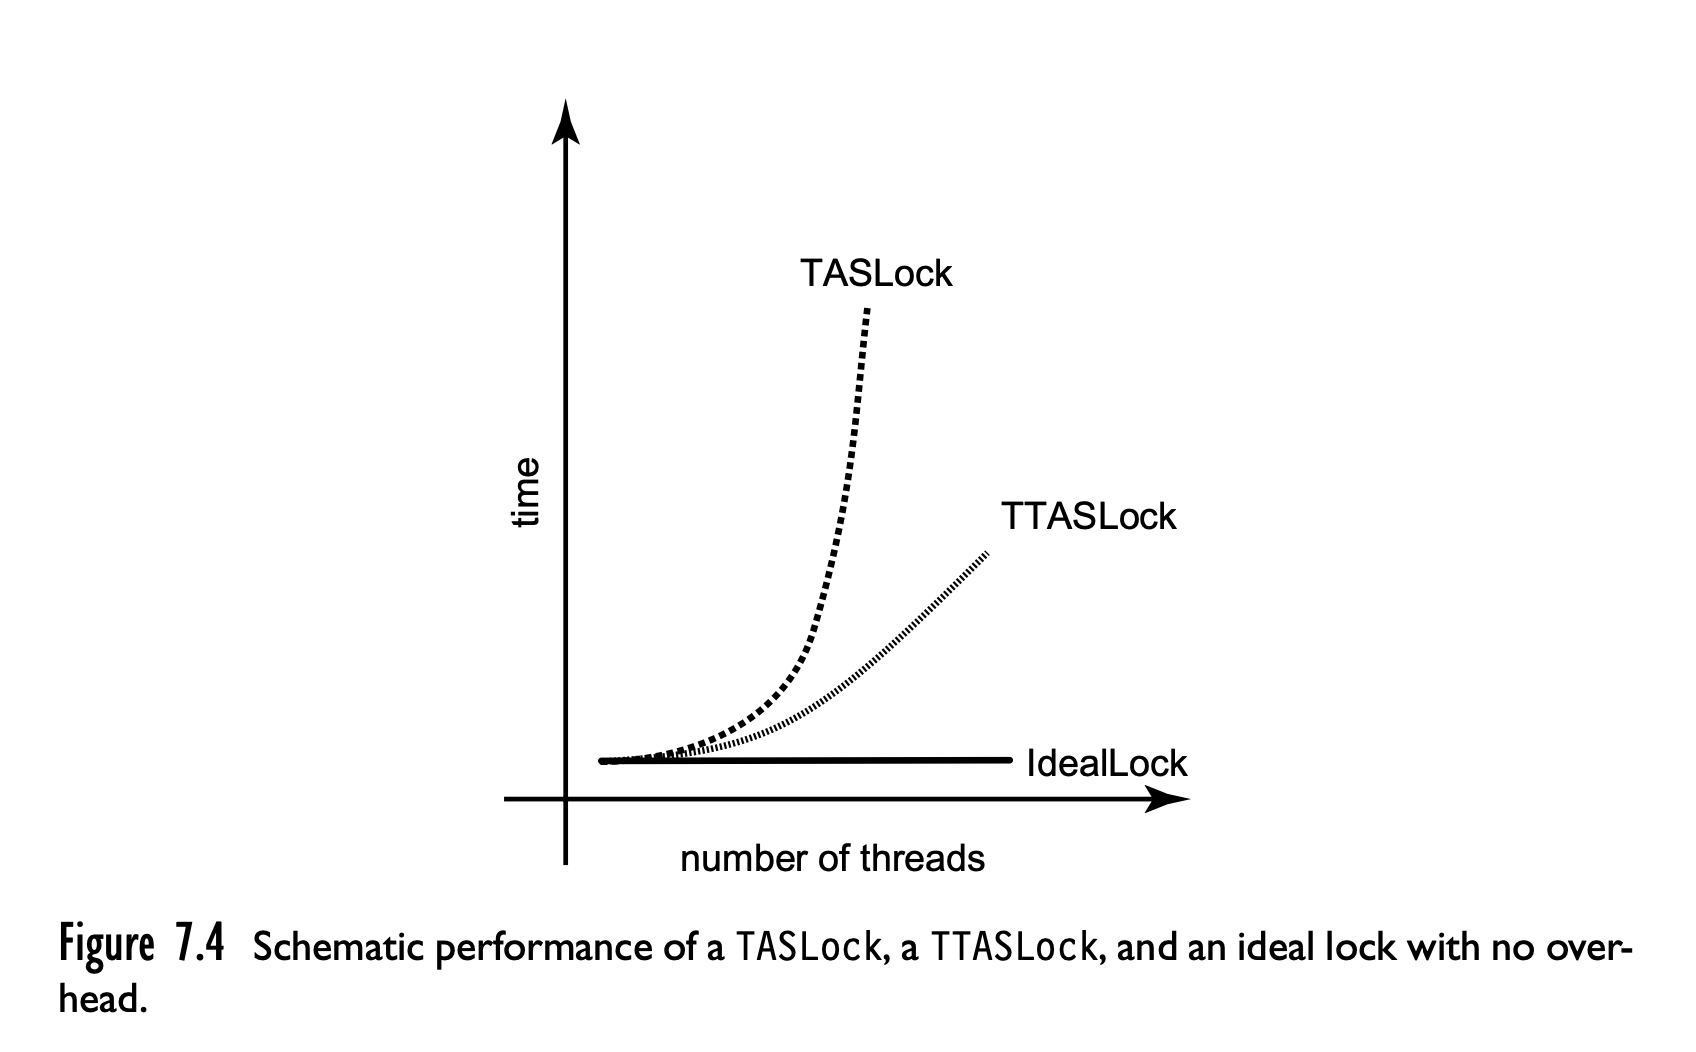
\includegraphics[width=\textwidth]{figure/plot_theory.png}
             \caption{Expected results}
             \label{fig:TASvTTAS_expected}
         \end{subfigure}
         \vfill
         \begin{subfigure}[b]{0.8\textwidth}
             \centering
             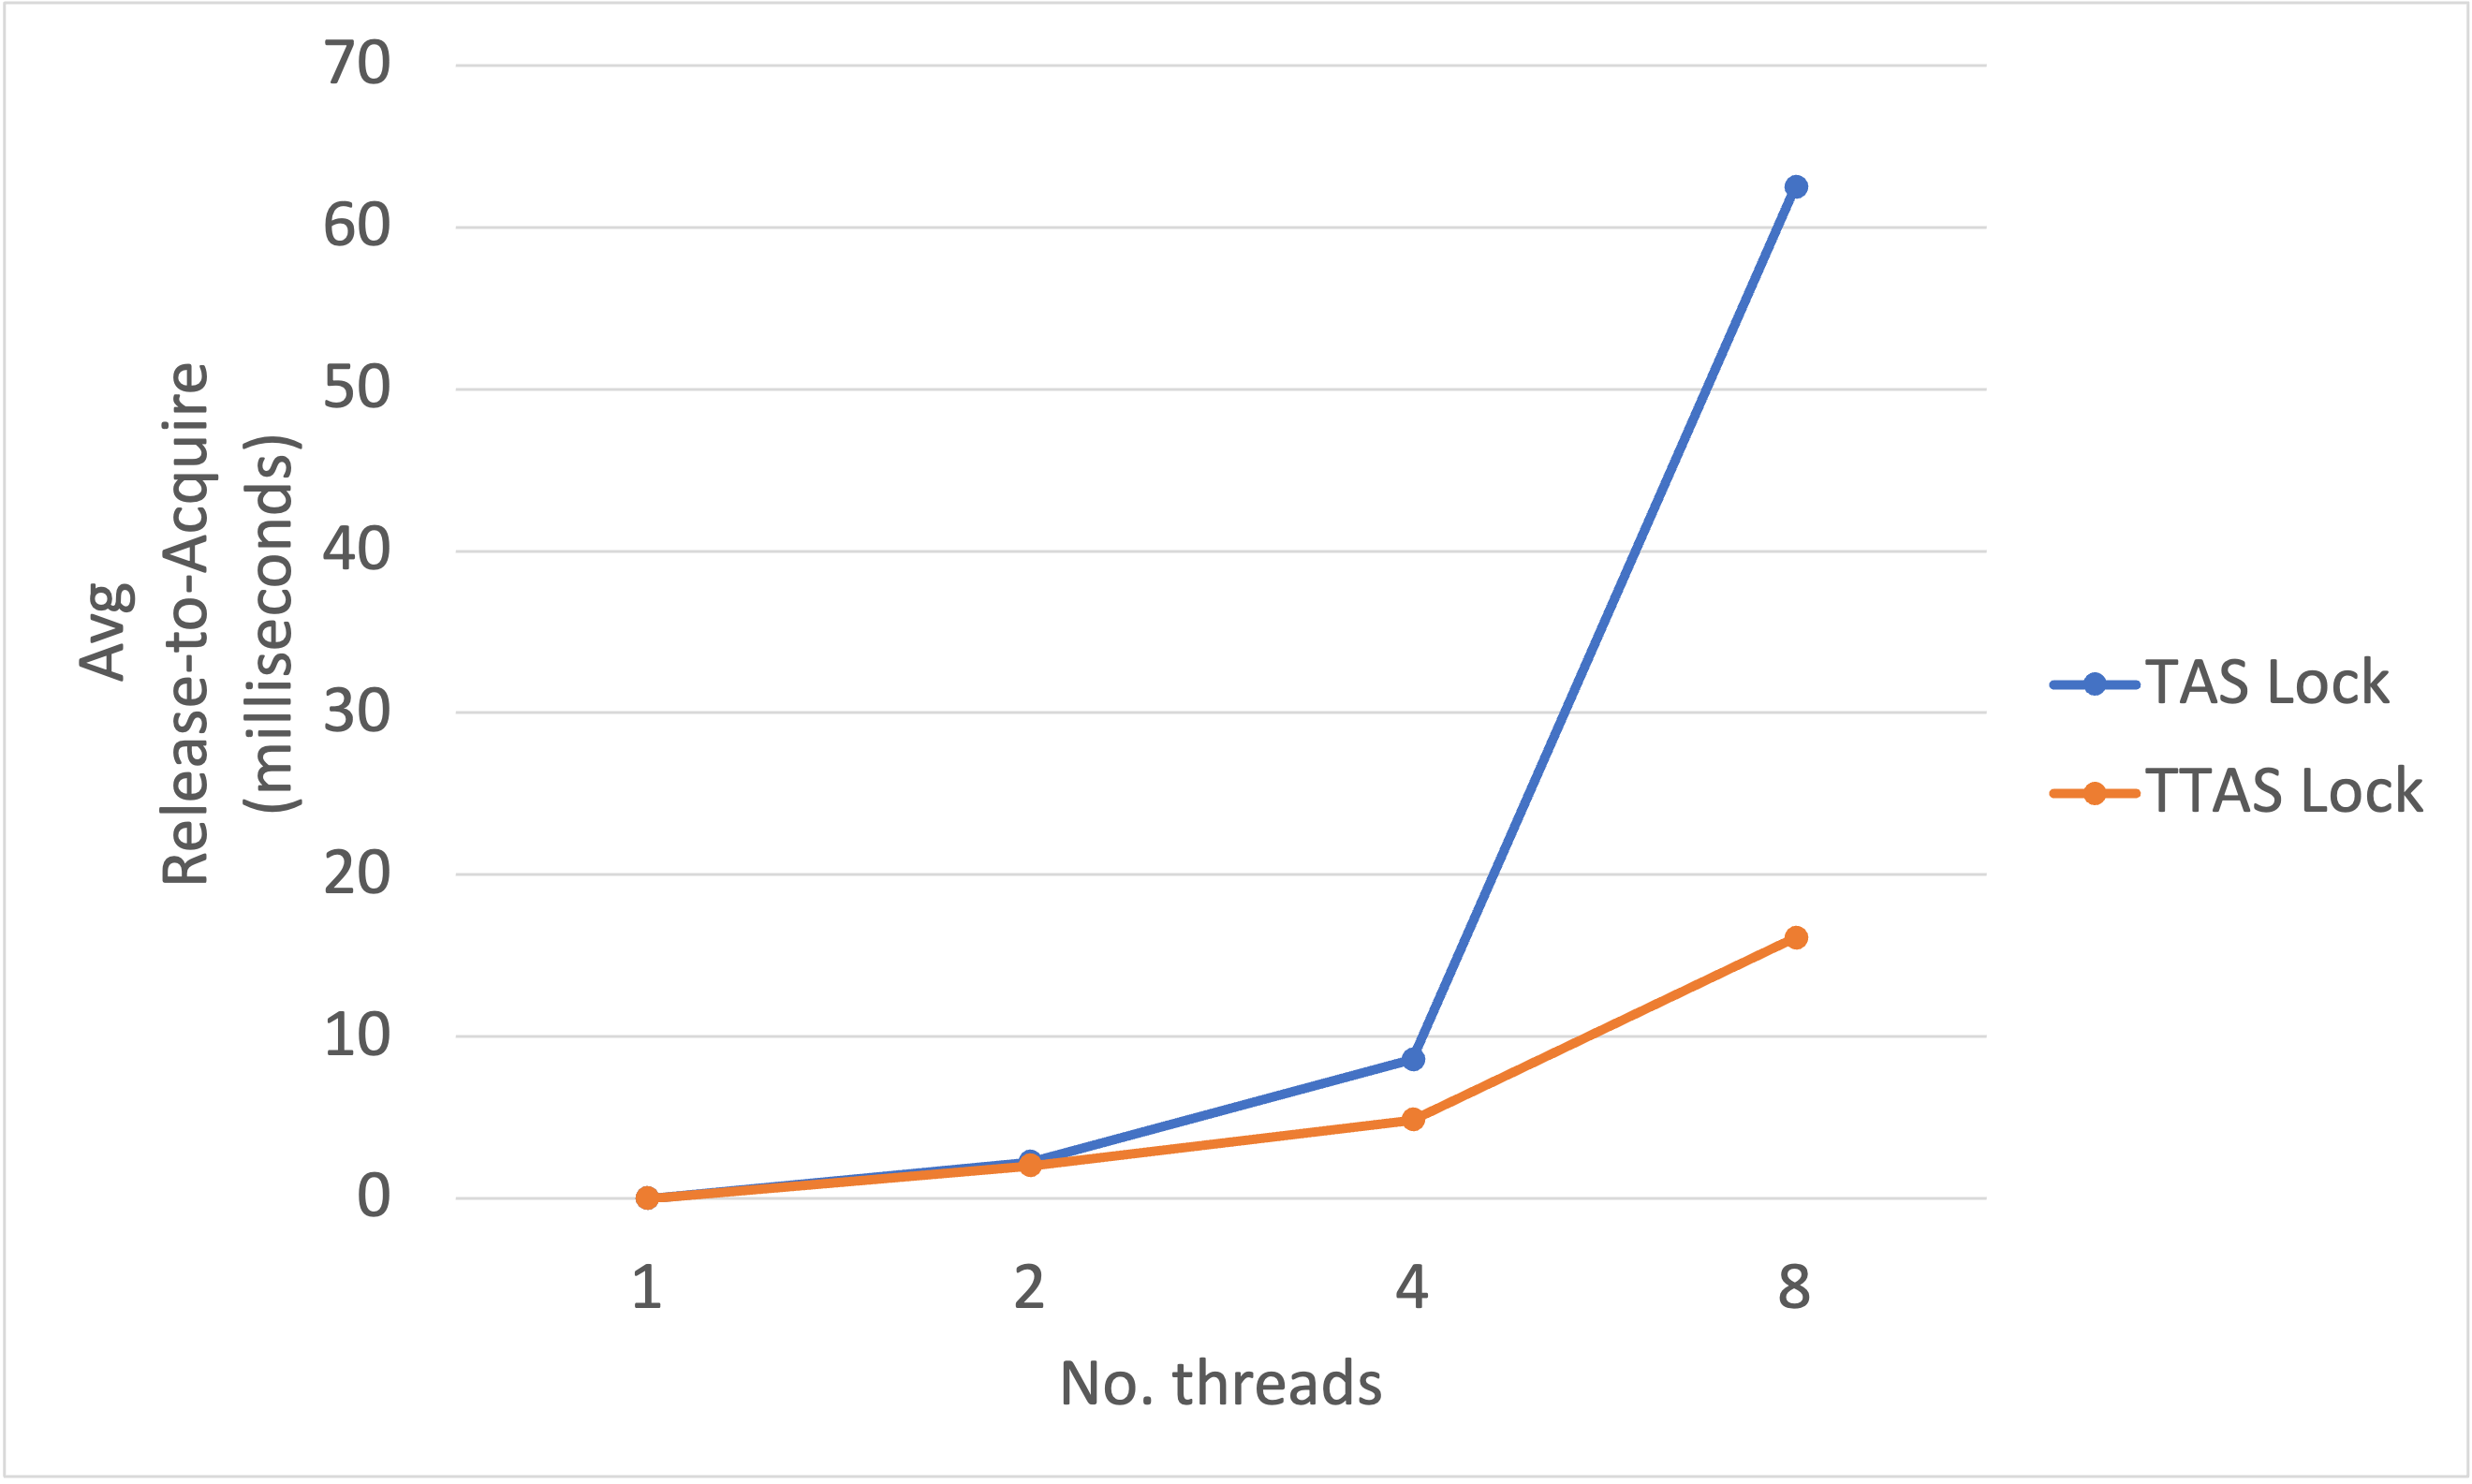
\includegraphics[width=\textwidth]{figure/correct_plot.png}
             \caption{Experimental results}
             \label{fig:TASvTTAS_experiment}
         \end{subfigure}
            \caption{Exercise 3.1 part 3}
            \label{fig:TASvTTAS_theory_v_practice}
        \end{figure}
    \end{enumerate}
\end{solution}

% \glsxtrshort{qm};
